% =============================================================================
% Trump Venezuela Press Conference
% Political Discourse Analysis
% Author: Antoine Lemor
% Date: January 2026
% =============================================================================

\documentclass[aspectratio=169,12pt]{beamer}

\usetheme{default}
\usecolortheme{default}

% Remove navigation symbols
\setbeamertemplate{navigation symbols}{}

% Colors - refined palette
\definecolor{bglight}{RGB}{250, 250, 252}
\definecolor{primary}{RGB}{30, 41, 59}
\definecolor{accent}{RGB}{59, 130, 246}
\definecolor{danger}{RGB}{239, 68, 68}
\definecolor{success}{RGB}{34, 197, 94}
\definecolor{muted}{RGB}{148, 163, 184}
\definecolor{subtle}{RGB}{226, 232, 240}

% Beamer colors
\setbeamercolor{background canvas}{bg=bglight}
\setbeamercolor{frametitle}{fg=primary}
\setbeamercolor{title}{fg=primary}
\setbeamercolor{subtitle}{fg=muted}
\setbeamercolor{author}{fg=primary}
\setbeamercolor{date}{fg=muted}
\setbeamercolor{section in toc}{fg=primary}
\setbeamercolor{itemize item}{fg=accent}
\setbeamercolor{itemize subitem}{fg=accent}
\setbeamercolor{enumerate item}{fg=accent}

% Fonts
\setbeamerfont{title}{size=\LARGE, series=\bfseries}
\setbeamerfont{subtitle}{size=\normalsize}
\setbeamerfont{frametitle}{size=\large, series=\bfseries}
\setbeamerfont{framesubtitle}{size=\small}

% Frame title format
\setbeamertemplate{frametitle}{
    \vspace{0.8em}
    \insertframetitle
    \par
    \usebeamerfont{framesubtitle}\usebeamercolor[fg]{framesubtitle}\insertframesubtitle
    \vspace{0.3em}
    \textcolor{subtle}{\rule{\textwidth}{0.5pt}}
    \vspace{0.3em}
}

% Packages
\usepackage[utf8]{inputenc}
\usepackage[T1]{fontenc}
\usepackage{graphicx}
\usepackage{booktabs}
\usepackage{tikz}
\usepackage{xcolor}
\usepackage{fontawesome5}
\usepackage{hyperref}
\hypersetup{colorlinks=true,linkcolor=primary,urlcolor=accent}

\usetikzlibrary{calc,shapes,positioning,shadows}

\graphicspath{{../output/figures/}}

% Custom commands
\newcommand{\emphdata}[1]{\textbf{\textcolor{accent}{#1}}}
\newcommand{\emphwarn}[1]{\textbf{\textcolor{danger}{#1}}}
\newcommand{\emphok}[1]{\textbf{\textcolor{success}{#1}}}
\newcommand{\muted}[1]{\textcolor{muted}{#1}}
\newcommand{\figframe}[1]{%
    \begin{tikzpicture}
        \node[inner sep=0pt] (fig) {#1};
        \draw[subtle, line width=0.5pt, rounded corners=2pt]
            ($(fig.south west)+(-2pt,-2pt)$) rectangle ($(fig.north east)+(2pt,2pt)$);
    \end{tikzpicture}%
}

% Analysis counter
\newcounter{analysisnum}
\setcounter{analysisnum}{0}

% For conditional check
\usepackage{xstring}

% Section page
\AtBeginSection[]{
  \IfStrEq{\insertsectionhead}{Conclusion}{%
    % Conclusion section - no analysis number
    \begin{frame}
    \vfill
    \centering
    \begin{tikzpicture}
      \node[fill=white, rounded corners=8pt, inner sep=20pt, drop shadow={shadow xshift=1pt, shadow yshift=-1pt, opacity=0.1}] {
        \begin{minipage}{0.6\textwidth}
          \centering
          {\LARGE\bfseries\textcolor{primary}{\insertsectionhead}}
        \end{minipage}
      };
    \end{tikzpicture}
    \vfill
    \end{frame}
  }{%
    % Regular analysis section
    \stepcounter{analysisnum}
    \begin{frame}
    \vfill
    \centering
    
\begin{tikzpicture}
      \node[fill=white, rounded corners=8pt, inner sep=20pt, drop shadow={shadow xshift=1pt, shadow yshift=-1pt, opacity=0.1}] {
        \begin{minipage}{0.6\textwidth}
          \centering
          \textcolor{muted}{\small ANALYSIS \#\theanalysisnum}\\[0.5em]
          {\LARGE\bfseries\textcolor{primary}{\insertsectionhead}}
        \end{minipage}
      };
    \end{tikzpicture}
    \vfill
    \end{frame}
  }
}

% Metadata
\title{Trump and Venezuela}
\subtitle{What the analysis of the January 3, 2026 press conference reveals}

\date{January 3, 2026}
\institute{}

\begin{document}

% =============================================================================
% TITLE
% =============================================================================
\begin{frame}[plain]
    \vfill
    \begin{center}
        \begin{tikzpicture}
            \node[fill=white, rounded corners=12pt, inner sep=30pt, drop shadow={shadow xshift=2pt, shadow yshift=-2pt, opacity=0.15}] {
                \begin{minipage}{0.75\textwidth}
                    \centering
                    {\small\textcolor{accent}{\faChartBar\ NLP \& political science}}\\[1em]
                    {\LARGE\bfseries\textcolor{primary}{Trump and Venezuela}}\\[0.8em]
                    {\normalsize\textcolor{muted}{What the analysis of the \\January 3, 2026 press conference reveals}}\\[1.5em]
                    \textcolor{subtle}{\rule{0.3\textwidth}{0.5pt}}\\[1.2em]
                    {\footnotesize\textcolor{muted}{January 5, 2026}}
                \end{minipage}
            };
        \end{tikzpicture}
    \end{center}
    \vfill
\end{frame}

% =============================================================================
% INTRODUCTION
% =============================================================================
\begin{frame}[c]{A press conference, four speakers}
    \centering
    \begin{columns}[c]
        \begin{column}{0.60\textwidth}
            \begin{tikzpicture}
                \node[fill=white, rounded corners=6pt, inner sep=15pt, drop shadow={opacity=0.08}] {
                    \begin{minipage}{0.85\textwidth}
                        {\large\bfseries January 3, 2026}\\[0.8em]
                        White House press conference following the military operation in Venezuela.\\[1.5em]
                        \muted{\footnotesize \faDatabase\ 858 annotated sentences}\\
                        \muted{\footnotesize \faNewspaper\ Associated Press transcript}\\
                        \muted{\footnotesize \faYoutube\ \href{https://www.youtube.com/watch?v=ezYNnFETXk0}{Source video}}
                    \end{minipage}
                };
            \end{tikzpicture}
        \end{column}
        \begin{column}{0.40\textwidth}
            \begin{tikzpicture}[every node/.style={inner sep=8pt}]
                \node[fill=white, rounded corners=4pt] at (0,0) {
                    \begin{tabular}{cl}
                        \textcolor{red!80!black}{\faSquare} & \textbf{Donald Trump} \\[-0.2em]
                        & \muted{\scriptsize President} \\[0.6em]
                        \textcolor{blue!70!black}{\faSquare} & \textbf{Marco Rubio} \\[-0.2em]
                        & \muted{\scriptsize Secretary of State} \\[0.6em]
                        \textcolor{green!60!black}{\faSquare} & \textbf{Pete Hegseth} \\[-0.2em]
                        & \muted{\scriptsize Secretary of Defense} \\[0.6em]
                        \textcolor{purple!70!black}{\faSquare} & \textbf{Dan Caine} \\[-0.2em]
                        & \muted{\scriptsize Chairman Joint Chiefs} \\
                    \end{tabular}
                };
            \end{tikzpicture}
        \end{column}
    \end{columns}
\end{frame}

% -----------------------------------------------------------------------------
\begin{frame}{Methodology}
    \vspace{0.5em}

    \centering
    \begin{tikzpicture}[
        node distance=1.2cm,
        box/.style={rectangle, rounded corners=6pt, minimum width=2.6cm, minimum height=1.2cm, align=center, font=\scriptsize},
        arrow/.style={->, >=stealth, thick, muted}
    ]
        % Boxes
        \node[box, fill=accent!15] (video) {\faYoutube\ \textbf{Video}\\[0.1em]\muted{\tiny AP}};
        \node[box, fill=success!15, right=of video] (transcription) {\faFile\ \textbf{Transcription}\\[0.1em]\muted{\tiny 858 sentences}};
        \node[box, fill=danger!15, right=of transcription] (annotation) {\faTags\ \textbf{Annotation}\\[0.1em]\muted{\tiny LLM}};
        \node[box, fill=purple!15, right=of annotation] (analyse) {\faChartBar\ \textbf{Analysis}};

        % Arrows
        \draw[arrow] (video) -- (transcription);
        \draw[arrow] (transcription) -- (annotation);
        \draw[arrow] (annotation) -- (analyse);
    \end{tikzpicture}

    \vspace{1.5em}

    \begin{tikzpicture}
        \node[fill=white, rounded corners=6pt, inner sep=15pt, drop shadow={opacity=0.08}] {
            \begin{minipage}{0.85\textwidth}
                \begin{tabular}{ll}
                    \faCode\ \textbf{Transcription} & \muted{\small\faGithub\ \href{https://github.com/antoinelemor/Transcribe-tool}{antoinelemor/Transcribe-tool}} \\[0.8em]
                    \faRobot\ \textbf{LLM Annotation} & \muted{\small\faGithub\ \href{https://github.com/antoinelemor/LLM_Tool}{antoinelemor/LLM\_Tool}} \\[0.8em]
                    \faPython\ \textbf{Analysis} & \muted{\small\faGithub\ \href{https://github.com/antoinelemor/nlp-pol}{antoinelemor/nlp-pol}}
                \end{tabular}
            \end{minipage}
        };
    \end{tikzpicture}
\end{frame}

% =============================================================================
% PART 1: RHETORICAL POSTURE
% =============================================================================
\section{What rhetorical posture adopted?}

% -----------------------------------------------------------------------------
{
\setbeamertemplate{navigation symbols}{}
\begin{frame}[plain]
    \begin{tikzpicture}[remember picture,overlay]
        \node[anchor=center] at (current page.center) {
            \includegraphics[width=0.95\paperwidth,height=0.92\paperheight,keepaspectratio]{fig1_posture_index_en.png}
        };
    \end{tikzpicture}
\end{frame}
}

% -----------------------------------------------------------------------------
{
\begin{frame}[plain]
    \begin{tikzpicture}[remember picture,overlay]
        \node[anchor=center] at (current page.center) {
            \includegraphics[width=0.95\paperwidth,height=0.92\paperheight,keepaspectratio]{fig2_posture_timeline_en.png}
        };
    \end{tikzpicture}
\end{frame}
}

% -----------------------------------------------------------------------------
\begin{frame}{Finding: Trump is not the most aggressive}
    \vspace{-1.7em}

    \begin{columns}[T]
        \begin{column}{0.52\textwidth}
            \begin{tikzpicture}
                \node[fill=white, rounded corners=6pt, inner sep=15pt, drop shadow={opacity=0.08}] {
                    \begin{minipage}{0.9\textwidth}
                        Contrary to the usual image, \textbf{Trump} adopts a \emphdata{moderate} tone.\\[1em]

                        The most aggressive?\\[0.5em]
                        \begin{itemize}
                            \item[\faExclamationTriangle] \emphwarn{Pete Hegseth} \muted{(-0.64)}
                            \item[\faExclamationTriangle] \emphwarn{Marco Rubio} \muted{(-0.49)}
                        \end{itemize}

                        \vspace{1em}
                        \muted{\small Joint Chiefs Chairman Caine remains neutral, he describes and doesn't justify.}
                    \end{minipage}
                };
            \end{tikzpicture}
        \end{column}
        \begin{column}{0.45\textwidth}
            \centering
            \vspace{1.5em}

            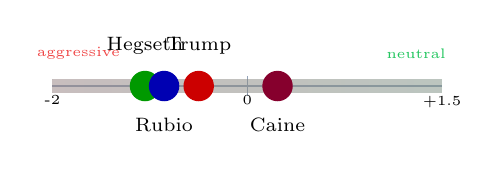
\begin{tikzpicture}[scale=1.1]
                % Axis
                \draw[muted, thick] (0,0) -- (4.5,0);
                \draw[muted] (2.25,-0.12) -- (2.25,0.12);

                % Labels
                \node[below, font=\tiny] at (0,0) {-2};
                \node[below, font=\tiny] at (2.25,0) {0};
                \node[below, font=\tiny] at (4.5,0) {+1.5};
                \node[above, font=\tiny, danger] at (0.3,0.2) {aggressive};
                \node[above, font=\tiny, success] at (4.2,0.2) {neutral};

                % Gradient background
                \fill[left color=danger!20, right color=success!20, opacity=0.3]
                    (0,-0.08) rectangle (4.5,0.08);

                % Markers with labels
                \fill[green!60!black] (1.07,0) circle (5pt);
                \node[above=8pt, font=\scriptsize] at (1.07,0) {Hegseth};

                \fill[blue!70!black] (1.29,0) circle (5pt);
                \node[below=8pt, font=\scriptsize] at (1.29,0) {Rubio};

                \fill[red!80!black] (1.69,0) circle (5pt);
                \node[above=8pt, font=\scriptsize] at (1.69,0) {Trump};

                \fill[purple!70!black] (2.60,0) circle (5pt);
                \node[below=8pt, font=\scriptsize] at (2.60,0) {Caine};
            \end{tikzpicture}

            \vspace{2em}

            \begin{tikzpicture}
                \node[fill=white, rounded corners=4pt, inner sep=10pt] {
                    \footnotesize
                    \begin{tabular}{lr}
                        \textcolor{green!60!black}{\faCircle} Hegseth & \textbf{-0.64} \\
                        \textcolor{blue!70!black}{\faCircle} Rubio & \textbf{-0.49} \\
                        \textcolor{red!80!black}{\faCircle} Trump & \textbf{-0.27} \\
                        \textcolor{purple!70!black}{\faCircle} Caine & \textbf{+0.15} \\
                    \end{tabular}
                };
            \end{tikzpicture}
        \end{column}
    \end{columns}
\end{frame}

\section{What topics raised by each speaker?}

% -----------------------------------------------------------------------------

% -----------------------------------------------------------------------------
{
\begin{frame}[plain]
    \begin{tikzpicture}[remember picture,overlay]
        \node[anchor=center] at (current page.center) {
            \includegraphics[width=0.95\paperwidth,height=0.92\paperheight,keepaspectratio]{fig6_topics_speakers_en.png}
        };
    \end{tikzpicture}
\end{frame}
}

% -----------------------------------------------------------------------------
\begin{frame}{Finding: a very clear division of roles}
    \vspace{-1.9em}

    \begin{columns}[T]
        \begin{column}{0.48\textwidth}
            \begin{tikzpicture}
                \node[fill=white, rounded corners=6pt, inner sep=12pt, drop shadow={opacity=0.08}] {
                    \begin{minipage}{0.9\textwidth}
                        {\large\textcolor{red!80!black}{\faSquare}\ \textbf{Trump}} \muted{\small n=489}\\[0.5em]
                        Security threat \emphdata{25\%}\\
                        Military operation 19\%\\
                        Economy/Oil 15\%\\
                        \muted{Humanitarian 7\%}
                    \end{minipage}
                };
            \end{tikzpicture}

            \vspace{0.8em}

            \begin{tikzpicture}
                \node[fill=white, rounded corners=6pt, inner sep=12pt, drop shadow={opacity=0.08}] {
                    \begin{minipage}{0.9\textwidth}
                        {\large\textcolor{green!60!black}{\faSquare}\ \textbf{Hegseth}} \muted{\small n=28}\\[0.5em]
                        Military operation \emphwarn{57\%}\\
                        Security threat 36\%\\
                        \emphwarn{Humanitarian 0\%}
                    \end{minipage}
                };
            \end{tikzpicture}
        \end{column}
        \begin{column}{0.48\textwidth}
            \begin{tikzpicture}
                \node[fill=white, rounded corners=6pt, inner sep=12pt, drop shadow={opacity=0.08}] {
                    \begin{minipage}{0.9\textwidth}
                        {\large\textcolor{blue!70!black}{\faSquare}\ \textbf{Rubio}} \muted{\small n=48}\\[0.5em]
                        Diplomacy \emphdata{40\%}\\
                        Legal/Justice 21\%\\
                        Security threat 17\%\\
                        \emphwarn{Humanitarian 0\%}
                    \end{minipage}
                };
            \end{tikzpicture}

            \vspace{0.8em}

            \begin{tikzpicture}
                \node[fill=white, rounded corners=6pt, inner sep=12pt, drop shadow={opacity=0.08}] {
                    \begin{minipage}{0.9\textwidth}
                        {\large\textcolor{purple!70!black}{\faSquare}\ \textbf{Caine}} \muted{\small n=67}\\[0.5em]
                        Military operation \emphdata{96\%}\\
                        \muted{Technical, factual}
                    \end{minipage}
                };
            \end{tikzpicture}
        \end{column}
    \end{columns}

    \vspace{0.8em}

    \centering
    
\begin{tikzpicture}
        \node[fill=accent!10, rounded corners=4pt, inner sep=8pt] {
            \small\textcolor{primary}{Only Trump mentions humanitarian issues. Hegseth and Rubio: \textbf{never}.}
        };
    \end{tikzpicture}
\end{frame}

% -----------------------------------------------------------------------------
\begin{frame}{Interpretation: an imperialist justification}
    \vspace{-1.7em}
    \vfill
    \centering
    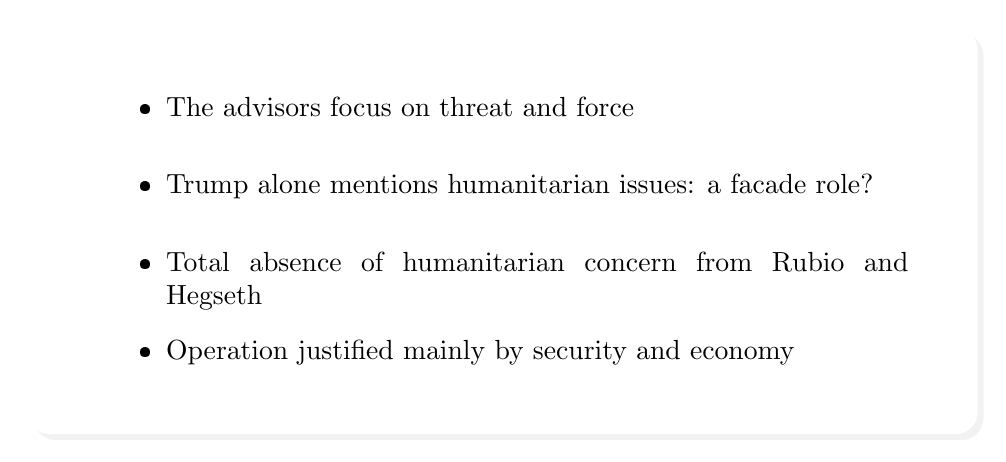
\begin{tikzpicture}
        \node[fill=white, rounded corners=8pt, inner sep=25pt, drop shadow={opacity=0.1}] {
            \begin{minipage}{0.85\textwidth}
                \begin{itemize}
                    \item The advisors focus on threat and force
                    \vspace{0.8em}
                    \item Trump alone mentions humanitarian issues: a facade role?
                    \vspace{0.8em}
                    \item Total absence of humanitarian concern from Rubio and Hegseth
                    \item Operation justified mainly by security and economy
                \end{itemize}
            \end{minipage}
        };
    \end{tikzpicture}
    \vfill
\end{frame}

\section{The US against the rest of the world?}

% -----------------------------------------------------------------------------


% -----------------------------------------------------------------------------
{
\begin{frame}[plain]
    \begin{tikzpicture}[remember picture,overlay]
        \node[anchor=center] at (current page.center) {
            \includegraphics[width=0.95\paperwidth,height=0.92\paperheight,keepaspectratio]{fig7_us_vs_them_en.png}
        };
    \end{tikzpicture}
\end{frame}
}

% -----------------------------------------------------------------------------
\begin{frame}{Finding: a strongly Manichean discourse}
    \vspace{-1.5em}

    \begin{columns}[T]
        \begin{column}{0.48\textwidth}
            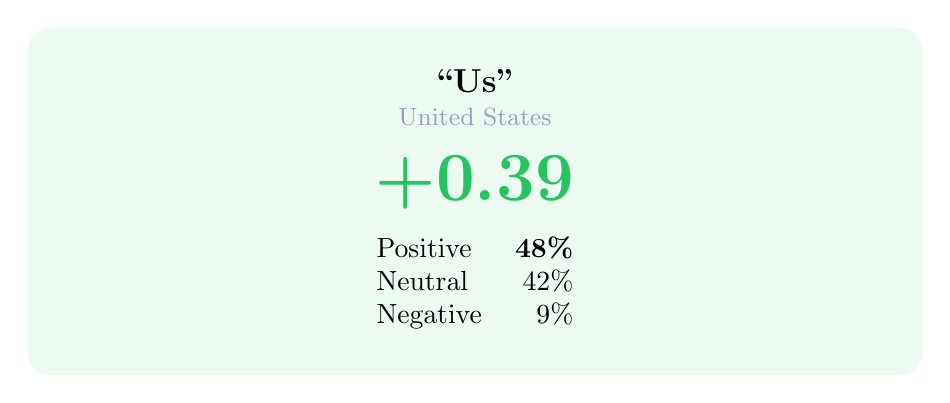
\begin{tikzpicture}
                \node[fill=success!8, rounded corners=8pt, inner sep=15pt] {
                    \begin{minipage}{0.85\textwidth}
                        \centering
                        {\large\bfseries ``Us''}\\
                        \muted{\small United States}\\[1em]
                        {\Huge\textcolor{success}{\textbf{+0.39}}}\\[0.8em]
                        \begin{tabular}{lr}
                            Positive & \textbf{48\%} \\
                            Neutral & 42\% \\
                            Negative & 9\% \\
                        \end{tabular}
                    \end{minipage}
                };
            \end{tikzpicture}
        \end{column}
        \begin{column}{0.48\textwidth}
            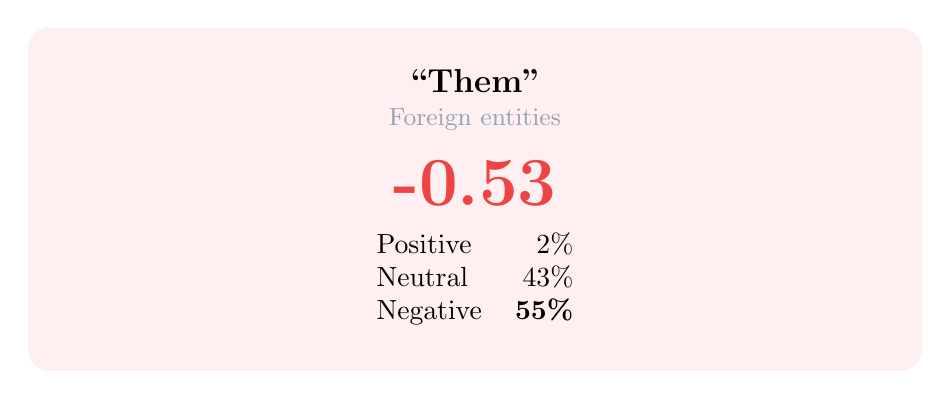
\begin{tikzpicture}
                \node[fill=danger!8, rounded corners=8pt, inner sep=15pt] {
                    \begin{minipage}{0.85\textwidth}
                        \centering
                        {\large\bfseries ``Them''}\\
                        \muted{\small Foreign entities}\\[1em]
                        {\Huge\textcolor{danger}{\textbf{-0.53}}}\\[0.8em]
                        \begin{tabular}{lr}
                            Positive & 2\% \\
                            Neutral & 43\% \\
                            Negative & \textbf{55\%} \\
                        \end{tabular}
                    \end{minipage}
                };
            \end{tikzpicture}
        \end{column}
    \end{columns}

    \vspace{0.2em}

    \centering
    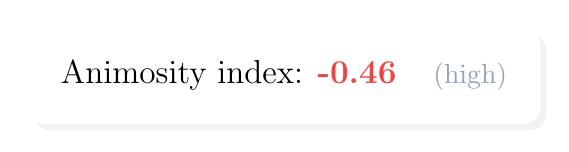
\begin{tikzpicture}
        \node[fill=white, rounded corners=6pt, inner sep=12pt, drop shadow={opacity=0.1}] {
            {\large Animosity index: \emphwarn{-0.46}} \quad \muted{(high)}
        };
    \end{tikzpicture}
\end{frame}

% -----------------------------------------------------------------------------
\begin{frame}{Interpretation: an imperialist isolationism?}
    \vspace{-1.7em}
    \vfill
    \centering
    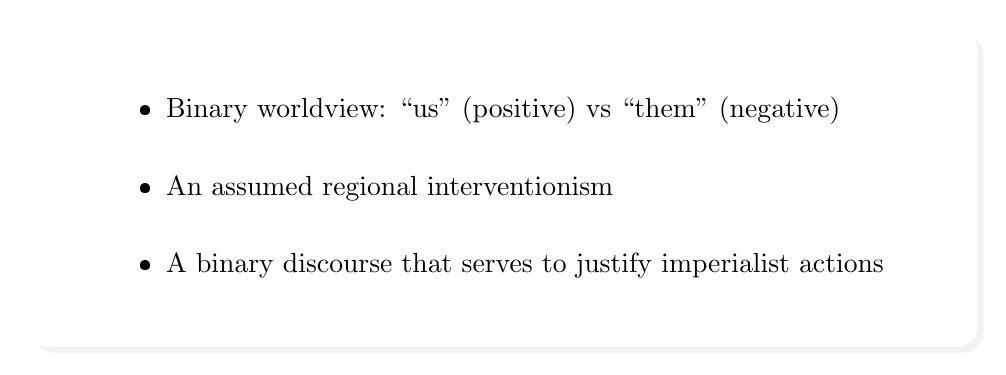
\begin{tikzpicture}
        \node[fill=white, rounded corners=8pt, inner sep=25pt, drop shadow={opacity=0.1}] {
            \begin{minipage}{0.85\textwidth}
                \begin{itemize}
                    \item Binary worldview: ``us'' (positive) vs ``them'' (negative)
                    \vspace{0.8em}
                    \item An assumed regional interventionism
                    \vspace{0.8em}
                    \item A binary discourse that serves to justify imperialist actions
                \end{itemize}
            \end{minipage}
        };
    \end{tikzpicture}
    \vfill
\end{frame}

% =============================================================================
% PART 2: Q&A ANALYSIS
% =============================================================================
\section{Facing journalists}

% -----------------------------------------------------------------------------
{
\begin{frame}[plain]
    \begin{tikzpicture}[remember picture,overlay]
        \node[anchor=center] at (current page.center) {
            \includegraphics[width=0.95\paperwidth,height=0.92\paperheight,keepaspectratio]{fig3_responses_en.png}
        };
    \end{tikzpicture}
\end{frame}
}

% -----------------------------------------------------------------------------
\begin{frame}{Finding: rarely direct answers}
    \vspace{-1em}

    \begin{columns}[c]
        \begin{column}{0.45\textwidth}
            \centering
            
\begin{tikzpicture}
                \node[fill=danger!10, rounded corners=12pt, inner sep=25pt] {
                    \begin{minipage}{0.7\textwidth}
                        \centering
                        {\fontsize{48}{52}\selectfont\textcolor{danger}{\textbf{72\%}}}\\[0.5em]
                        {\large \textbf{partial} answers}
                    \end{minipage}
                };
            \end{tikzpicture}

            \vspace{1.5em}

            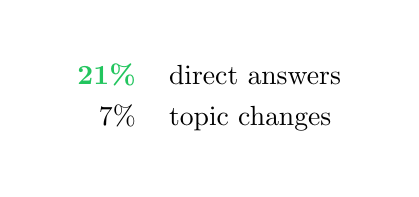
\begin{tikzpicture}
                \node[fill=white, rounded corners=6pt, inner sep=12pt] {
                    \begin{tabular}{rl}
                        \emphok{21\%} & direct answers \\[0.3em]
                        7\% & topic changes \\
                    \end{tabular}
                };
            \end{tikzpicture}
        \end{column}
        \begin{column}{0.5\textwidth}
            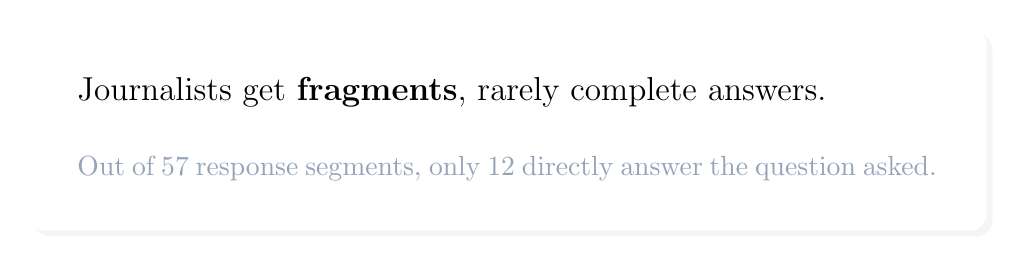
\begin{tikzpicture}
                \node[fill=white, rounded corners=6pt, inner sep=18pt, drop shadow={opacity=0.08}] {
                    \begin{minipage}{0.9\textwidth}
                        {\large Journalists get \textbf{fragments}, rarely complete answers.}\\[1.5em]
                        \muted{Out of 57 response segments, only 12 directly answer the question asked.}
                    \end{minipage}
                };
            \end{tikzpicture}
        \end{column}
    \end{columns}
\end{frame}

% -----------------------------------------------------------------------------
{
\begin{frame}[plain]
    \begin{tikzpicture}[remember picture,overlay]
        \node[anchor=center] at (current page.center) {
            \includegraphics[width=0.95\paperwidth,height=0.92\paperheight,keepaspectratio]{fig5_progressive_en.png}
        };
    \end{tikzpicture}
\end{frame}
}

% -----------------------------------------------------------------------------
\begin{frame}{Finding: oil above all}
    \vspace{-0.5em}

    \centering
    {\large A revealing thematic gap}

    \vspace{0.8em}

    \begin{columns}[T]
        \begin{column}{0.48\textwidth}
            \begin{tikzpicture}
                \node[fill=accent!8, rounded corners=8pt, inner sep=15pt] {
                    \begin{minipage}{0.85\textwidth}
                        {\large\bfseries\faNewspaper\ Journalists}\\[0.8em]
                        \begin{enumerate}
                            \item Diplomacy
                            \item Governance
                            \item Legal / Justice
                        \end{enumerate}
                        \vspace{0.8em}
                        \muted{\small Questions about the \textit{how}}
                    \end{minipage}
                };
            \end{tikzpicture}
        \end{column}
        \begin{column}{0.48\textwidth}
            \begin{tikzpicture}
                \node[fill=danger!8, rounded corners=8pt, inner sep=15pt] {
                    \begin{minipage}{0.85\textwidth}
                        {\large\bfseries\faUser\ Trump answers}\\[0.8em]
                        \begin{enumerate}
                            \item \emphwarn{Economy / Oil}
                            \item Military operation
                            \item Diplomacy
                        \end{enumerate}
                        \vspace{0.8em}
                        \muted{\small Insistence on \textit{resources}}
                    \end{minipage}
                };
            \end{tikzpicture}
        \end{column}
    \end{columns}

    \vspace{1em}

    \centering
    
\begin{tikzpicture}
        \node[fill=white, rounded corners=6pt, inner sep=12pt, drop shadow={opacity=0.1}] {
            \large Trump focused on \textbf{resources} above all
        };
    \end{tikzpicture}
\end{frame}

% -----------------------------------------------------------------------------
{
\begin{frame}[plain]
    \begin{tikzpicture}[remember picture,overlay]
        \node[anchor=center] at (current page.center) {
            \includegraphics[width=0.95\paperwidth,height=0.92\paperheight,keepaspectratio]{fig4_evasion_en.png}
        };
    \end{tikzpicture}
\end{frame}
}

% -----------------------------------------------------------------------------
\begin{frame}{Finding: the ``how'' remains unanswered}
    \vspace{-1em}

    \centering
    {\large The most \textbf{avoided} topics are the most \textbf{concrete}}

    \vspace{1em}

    \begin{columns}[T]
        \begin{column}{0.48\textwidth}
            
\begin{tikzpicture}
                \node[fill=danger!8, rounded corners=6pt, inner sep=12pt] {
                    \begin{minipage}{0.85\textwidth}
                        \centering
                        {\Large\emphwarn{80\%}}\\[0.2em]
                        \textbf{Governance}\\
                        \muted{\footnotesize partial answer}
                    \end{minipage}
                };
            \end{tikzpicture}

            \vspace{0.6em}

            
\begin{tikzpicture}
                \node[fill=danger!7, rounded corners=6pt, inner sep=12pt] {
                    \begin{minipage}{0.85\textwidth}
                        \centering
                        {\Large\emphwarn{77\%}}\\[0.2em]
                        \textbf{Diplomacy}\\
                        \muted{\footnotesize partial answer}
                    \end{minipage}
                };
            \end{tikzpicture}
        \end{column}
        \begin{column}{0.48\textwidth}
            
\begin{tikzpicture}
                \node[fill=danger!6, rounded corners=6pt, inner sep=12pt] {
                    \begin{minipage}{0.85\textwidth}
                        \centering
                        {\Large\emphwarn{67\%}}\\[0.2em]
                        \textbf{Legal / Justice}\\
                        \muted{\footnotesize partial answer}
                    \end{minipage}
                };
            \end{tikzpicture}

            \vspace{0.6em}

            
\begin{tikzpicture}
                \node[fill=subtle, rounded corners=6pt, inner sep=12pt] {
                    \begin{minipage}{0.85\textwidth}
                        \centering
                        {\Large\emphwarn{33\%}}\\[0.2em]
                        \textbf{Economy / Oil}\\
                        \muted{\footnotesize topic change/defer to advisor}
                    \end{minipage}
                };
            \end{tikzpicture}
        \end{column}
    \end{columns}

    \vspace{1em}

    \muted{Only exception: US domestic politics (\emphok{92\%} direct answers)}
\end{frame}

% =============================================================================
% CONCLUSION
% =============================================================================
\section{Conclusion}

% -----------------------------------------------------------------------------
\begin{frame}{What the analysis reveals}
    \vspace{-1.3em}

    \begin{columns}[T]
        \begin{column}{0.48\textwidth}
            \begin{tikzpicture}
                \node[fill=white, rounded corners=8pt, inner sep=14pt, drop shadow={opacity=0.1}] {
                    \begin{minipage}{0.9\textwidth}
                        {\large\textcolor{accent}{\faUsers}\ \textbf{Delegated aggression}}\\[0.4em]
                        Trump moderate, advisors offensive. The president leads, pushed by his entourage.
                    \end{minipage}
                };
            \end{tikzpicture}

            \vspace{0.6em}

            \begin{tikzpicture}
                \node[fill=white, rounded corners=8pt, inner sep=14pt, drop shadow={opacity=0.1}] {
                    \begin{minipage}{0.9\textwidth}
                        {\large\textcolor{accent}{\faGlobe}\ \textbf{Clear imperialism}}\\[0.4em]
                        Assumed regional interventionism. Binary ``us'' vs ``them'' worldview.
                    \end{minipage}
                };
            \end{tikzpicture}
        \end{column}
        \begin{column}{0.48\textwidth}
            \begin{tikzpicture}
                \node[fill=white, rounded corners=8pt, inner sep=14pt, drop shadow={opacity=0.1}] {
                    \begin{minipage}{0.9\textwidth}
                        {\large\textcolor{accent}{\faOilCan}\ \textbf{Oil above all}}\\[0.4em]
                        Revealing thematic gap. Justified by resources, not humanitarian concerns.
                    \end{minipage}
                };
            \end{tikzpicture}

            \vspace{0.6em}

            
\begin{tikzpicture}
                \node[fill=white, rounded corners=8pt, inner sep=14pt, drop shadow={opacity=0.1}] {
                    \begin{minipage}{0.9\textwidth}
                        {\large\textcolor{accent}{\faQuestionCircle}\ \textbf{The future remains unclear}}\\[0.4em]
                        Governance, legality: no concrete plan for the aftermath.
                    \end{minipage}
                };
            \end{tikzpicture}
        \end{column}
    \end{columns}
\end{frame}

% -----------------------------------------------------------------------------
\begin{frame}[plain]
    \vfill
    \begin{center}
        \begin{tikzpicture}
            \node[fill=white, rounded corners=12pt, inner sep=30pt, drop shadow={opacity=0.15}] {
                \begin{minipage}{0.6\textwidth}
                    \centering
                    {\bfseries Antoine Lemor}\\[0.5em]
                    \muted{\small\faGithub\ \href{https://github.com/antoinelemor}{github.com/antoinelemor}}\\[1.5em]
                    \textcolor{subtle}{\rule{0.6\textwidth}{0.5pt}}\\[1.2em]
                    {\small Want to see the method and code?}\\[1em]
                    \begin{tabular}{@{}rl@{}}
                    \faChartBar\ \textbf{This analysis} & \muted{\small\href{https://github.com/antoinelemor/nlp-pol}{antoinelemor/nlp-pol}} \\[0.5em]
                    \faCode\ \textbf{Transcription} & \muted{\small\href{https://github.com/antoinelemor/Transcribe-tool}{antoinelemor/Transcribe-tool}} \\[0.5em]
                    \faRobot\ \textbf{LLM Annotation} & \muted{\small\href{https://github.com/antoinelemor/LLM_Tool}{antoinelemor/LLM\_Tool}}
                    \end{tabular}
                \end{minipage}
            };
        \end{tikzpicture}
    \end{center}
    \vfill
\end{frame}

\end{document}
